\documentclass{standalone}
\usepackage{tikz}
\usetikzlibrary{shapes.geometric, arrows.meta, positioning}
\usepackage{xcolor}
\definecolor{blue!50}{RGB}{50,100,200}
\definecolor{green!50}{RGB}{34,140,34}
\definecolor{orange!50}{RGB}{200,100,50}
\begin{document}
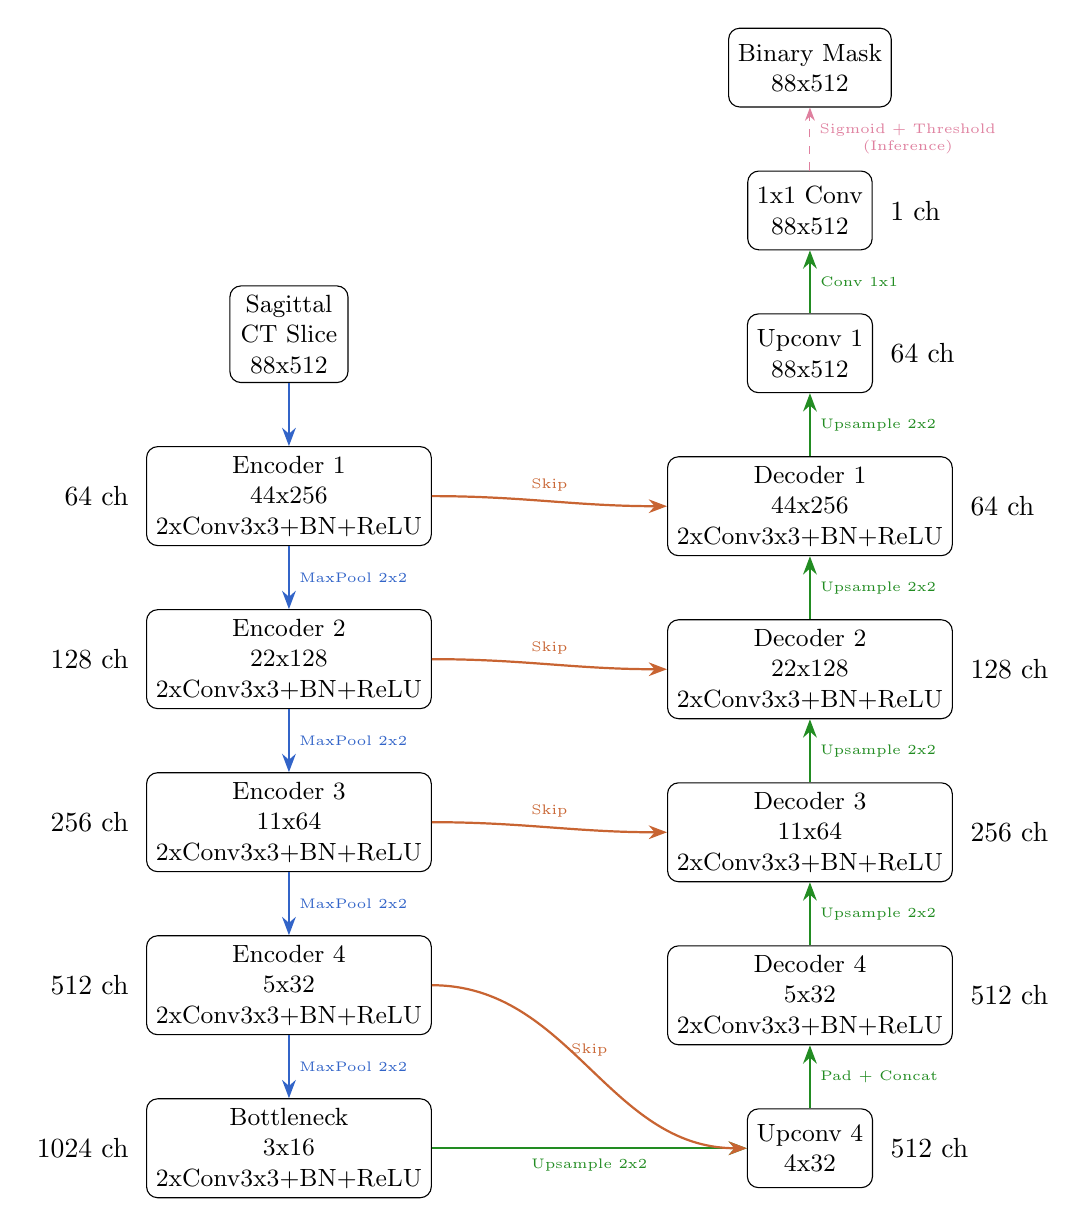
\begin{tikzpicture}[
    node distance=0.8cm and 0.8cm,
    box/.style={
        rectangle, 
        draw, 
        rounded corners, 
        minimum height=1cm, 
        minimum width=1.5cm, 
        align=center, 
        font=\small
    },
    encoderArrow/.style={-Stealth, thick, blue!50},
    decoderArrow/.style={-Stealth, thick, green!50},
    skipArrow/.style={-Stealth, thick, orange!50}
]
    % Encoder path (left side)
    \node[box] (input) at (0, 0) {Sagittal\\CT Slice\\88x512};
    \node[box, below=of input] (enc1) {Encoder 1\\44x256\\2xConv3x3+BN+ReLU};
    \node[box, below=of enc1] (enc2) {Encoder 2\\22x128\\2xConv3x3+BN+ReLU};
    \node[box, below=of enc2] (enc3) {Encoder 3\\11x64\\2xConv3x3+BN+ReLU};
    \node[box, below=of enc3] (enc4) {Encoder 4\\5x32\\2xConv3x3+BN+ReLU};
    \node[box, below=of enc4] (bottleneck) {Bottleneck\\3x16\\2xConv3x3+BN+ReLU};

    % Decoder path (right side)
    \node[box, right=4cm of bottleneck] (up4) {Upconv 4\\4x32};
    \node[box, above=of up4] (dec4) {Decoder 4\\5x32\\2xConv3x3+BN+ReLU};
    \node[box, above=of dec4] (dec3) {Decoder 3\\11x64\\2xConv3x3+BN+ReLU};
    \node[box, above=of dec3] (dec2) {Decoder 2\\22x128\\2xConv3x3+BN+ReLU};
    \node[box, above=of dec2] (dec1) {Decoder 1\\44x256\\2xConv3x3+BN+ReLU};
    \node[box, above=of dec1] (up1) {Upconv 1\\88x512};
    \node[box, above=of up1] (convlast) {1x1 Conv\\88x512};
    \node[box, above=of convlast] (output) {Binary Mask\\88x512};

    % Feature channels
    \node[left=0.1cm of enc1] {64 ch};
    \node[left=0.1cm of enc2] {128 ch};
    \node[left=0.1cm of enc3] {256 ch};
    \node[left=0.1cm of enc4] {512 ch};
    \node[left=0.1cm of bottleneck] {1024 ch};
    \node[right=0.1cm of up4] {512 ch};
    \node[right=0.1cm of dec4] {512 ch};
    \node[right=0.1cm of dec3] {256 ch};
    \node[right=0.1cm of dec2] {128 ch};
    \node[right=0.1cm of dec1] {64 ch};
    \node[right=0.1cm of up1] {64 ch};
    \node[right=0.1cm of convlast] {1 ch};

    % Data flow arrows
    \draw[encoderArrow] (input) -- (enc1);
    \draw[encoderArrow] (enc1) -- node[right, font=\tiny] {MaxPool 2x2} (enc2);
    \draw[encoderArrow] (enc2) -- node[right, font=\tiny] {MaxPool 2x2} (enc3);
    \draw[encoderArrow] (enc3) -- node[right, font=\tiny] {MaxPool 2x2} (enc4);
    \draw[encoderArrow] (enc4) -- node[right, font=\tiny] {MaxPool 2x2} (bottleneck);

    \draw[decoderArrow] (bottleneck) -- node[below, font=\tiny] {Upsample 2x2} (up4);
    \draw[decoderArrow] (up4) -- node[right, font=\tiny] {Pad + Concat} (dec4);
    \draw[decoderArrow] (dec4) -- node[right, font=\tiny] {Upsample 2x2} (dec3);
    \draw[decoderArrow] (dec3) -- node[right, font=\tiny] {Upsample 2x2} (dec2);
    \draw[decoderArrow] (dec2) -- node[right, font=\tiny] {Upsample 2x2} (dec1);
    \draw[decoderArrow] (dec1) -- node[right, font=\tiny] {Upsample 2x2} (up1);
    \draw[decoderArrow] (up1) -- node[right, font=\tiny] {Conv 1x1} (convlast);
    \draw[purple!50, dashed, -Stealth] (convlast) -- node[right, font=\tiny, align=center] {Sigmoid + Threshold\\(Inference)} (output);

    % Skip connections
    \draw[skipArrow] (enc4.east) to[out=0,in=180] node[above, font=\tiny] {Skip} (up4.west);
    \draw[skipArrow] (enc3.east) to[out=0,in=180] node[above, font=\tiny] {Skip} (dec3.west);
    \draw[skipArrow] (enc2.east) to[out=0,in=180] node[above, font=\tiny] {Skip} (dec2.west);
    \draw[skipArrow] (enc1.east) to[out=0,in=180] node[above, font=\tiny] {Skip} (dec1.west);
\end{tikzpicture}
\end{document}